\documentclass[11pt]{article}
\usepackage{geometry}
\geometry{a4paper, left=2.2cm, right=2.2cm, top=2.4cm, bottom=2.0cm, headheight=14.5pt}
\usepackage{fontspec}
% Fuente monoespaciada explícita: evita un glitch de renderizado (la "i"
% confundida con "1") que aparece en algunos visores de PDF con la fuente
% Latin Modern Mono descargada por defecto por tectonic.
\IfFontExistsTF{Consolas}{\setmonofont{Consolas}[Scale=0.92]}{}
\usepackage[spanish,es-noshorthands]{babel}
\usepackage{fancyvrb}
\usepackage{tikz}
\usepackage[most]{tcolorbox}
\usepackage{tabularx}
\newcolumntype{Y}{>{\raggedright\arraybackslash}X}
\usepackage{enumitem}
\usepackage{xcolor}
\usepackage{parskip}
\usepackage[hidelinks]{hyperref}
\usepackage{fancyhdr}
\usepackage{titlesec}
\usepackage{graphicx}

\setlength{\parindent}{0pt}
\setlength{\parskip}{4pt plus 1pt minus 1pt}
\setlist[enumerate]{leftmargin=*, itemsep=0.5mm}
\setlist[itemize]{leftmargin=*, itemsep=0.5mm}

% =========================================
% COLORES
% =========================================
\definecolor{azuloscuro}{RGB}{0,51,102}
\definecolor{verdealerta}{RGB}{0,128,0}
\definecolor{rojoalerta}{RGB}{180,0,0}
\definecolor{marcogris}{RGB}{170,170,170}
\definecolor{guialinea}{gray}{0.65}

% =========================================
% FORMATO DE SECCIONES
% =========================================
\titleformat{\section}{\Large\bfseries\color{azuloscuro}}{}{0em}{}[\vspace{-0.3em}\rule{\textwidth}{0.8pt}]
\titleformat{\subsection}{\large\bfseries\color{azuloscuro}}{}{0em}{}
\titleformat{\subsubsection}[runin]{\normalsize\bfseries\color{azuloscuro}}{}{0em}{}[.\quad]

% =========================================
% CAJAS --- SIEMPRE FONDO BLANCO (nunca relleno de color: se imprime en blanco y negro)
% =========================================
\newtcolorbox{cajacodigo}{
  colback=white, colframe=marcogris, boxrule=0.4pt,
  arc=1mm, left=3mm, right=3mm, top=1.5mm, bottom=1.5mm, breakable
}
% cajaescribe: caja en blanco para escribir código a mano, con líneas guía
% verticales punteadas que marcan cada nivel de indentación (ver "Regla de
% indentación" en la portada). Los xshift son fijos (no \foreach) para máxima
% robustez de compilación.
\newtcolorbox{cajaescribe}[1][]{
  enhanced,
  colback=white, colframe=marcogris, boxrule=0.6pt,
  arc=1mm, left=3mm, right=3mm, top=1.5mm, bottom=1.5mm,
  overlay={
    \draw[guialinea, dash pattern=on 1.5pt off 1.8pt, line width=0.3pt] ([xshift=0.8cm]frame.north west) -- ([xshift=0.8cm]frame.south west);
    \draw[guialinea, dash pattern=on 1.5pt off 1.8pt, line width=0.3pt] ([xshift=1.6cm]frame.north west) -- ([xshift=1.6cm]frame.south west);
    \draw[guialinea, dash pattern=on 1.5pt off 1.8pt, line width=0.3pt] ([xshift=2.4cm]frame.north west) -- ([xshift=2.4cm]frame.south west);
    \draw[guialinea, dash pattern=on 1.5pt off 1.8pt, line width=0.3pt] ([xshift=3.2cm]frame.north west) -- ([xshift=3.2cm]frame.south west);
    \draw[guialinea, dash pattern=on 1.5pt off 1.8pt, line width=0.3pt] ([xshift=4.0cm]frame.north west) -- ([xshift=4.0cm]frame.south west);
  },
  #1
}
\newtcolorbox{formulabox}[1][]{
  colback=white, colframe=azuloscuro, colbacktitle=white, coltitle=azuloscuro,
  fonttitle=\bfseries, title=#1, breakable, arc=1mm,
  left=3mm, right=3mm, top=1mm, bottom=1mm, toptitle=0.5mm, bottomtitle=0.5mm
}
\newtcolorbox{alertabox}[1][]{
  colback=white, colframe=rojoalerta, colbacktitle=white, coltitle=rojoalerta,
  fonttitle=\bfseries, title=#1, breakable, arc=1mm,
  left=3mm, right=3mm, top=1mm, bottom=1mm, toptitle=0.5mm, bottomtitle=0.5mm
}
\newtcolorbox{actitudbox}[1][]{
  colback=white, colframe=verdealerta, colbacktitle=white, coltitle=verdealerta,
  fonttitle=\bfseries, title=#1, breakable, arc=1mm,
  left=3mm, right=3mm, top=1mm, bottom=1mm, toptitle=0.5mm, bottomtitle=0.5mm
}

% =========================================
% ENCABEZADO
% =========================================
\pagestyle{fancy}
\fancyhf{}
\fancyfoot[C]{\thepage}
\renewcommand{\headrulewidth}{0.4pt}
\renewcommand{\footrulewidth}{0pt}
\lhead{\small Programación Python --- 4to Medio}
\rhead{\small Prof. Diego Vargas P.}

\begin{document}

% =========================================
% ENCABEZADO COMPACTO (sin portada de una hoja)
% =========================================
\noindent
\begin{minipage}[c]{0.11\textwidth}
    \IfFileExists{logo.png}{
\includegraphics[width=\linewidth]{logo.png}}{}
\end{minipage}%
\hspace{0.03\textwidth}%
\begin{minipage}[c]{0.82\textwidth}
    {\Large \textbf{EJERCITACIÓN --- CICLOS}}
\end{minipage}

\vspace{0.06cm}
\begin{actitudbox}[Objetivo y propósito de la sesión]
\textbf{Objetivo:} aplicar \texttt{for}+\texttt{range()}, \texttt{for} anidado, \texttt{while} y \texttt{continue}/\texttt{break} en problemas estilo evaluación, para llegar con seguridad a la Evaluación de Ciclos del jueves.

\vspace{1mm}
\textit{\textbf{Propósito:} hoy practicamos bajo las condiciones de la evaluación del jueves --- mismos tipos de problemas, mismo trabajo individual, pero sin nota. Practicar bajo esa presión controlada, y revisar juntos los errores al final, es lo que te permite llegar con más confianza al día real.}
\end{actitudbox}

\vspace{0.08cm}
\begin{center}
    \renewcommand{\arraystretch}{0.95}
    \begin{tabular}{rl}
        \textbf{Nombre:} & \rule{8.5cm}{0.4pt} \\
        \textbf{Fecha:}  & \rule{8.5cm}{0.4pt} \\
        \textbf{Curso:}  & \rule{8.5cm}{0.4pt}
    \end{tabular}
\end{center}

\vspace{0.1cm}

\begin{formulabox}[Instrucciones generales]
\begin{itemize}
  \item Esta sesión tiene \textbf{3 partes}: una Práctica Guiada (se resuelve en conjunto), 4 ítems cortos, y 2 programas de desarrollo.
  \item \textbf{No lleva nota.} Al terminar, revisamos juntos los errores más comunes.
  \item Escribe tu código \textbf{a mano, con letra clara} --- el profesor debe poder leerlo sin dudas.
  \item Si te equivocas, tacha con una línea y escribe al lado. No necesitas que quede perfecto, pero sí legible.
  \item Usa nombres de variables en \textbf{snake\_case en español}.
  \item Cuando un ítem pida un dato con \texttt{input()}, el enunciado siempre aclara si es un \textbf{número entero}, un \textbf{número con decimales}, o una \textbf{palabra exacta}.
  \item Si no terminas un ítem, deja lo que alcanzaste --- se revisa lo escrito tal como está.
  \item Trabajo individual, en las mismas condiciones que la evaluación real.
\end{itemize}
\end{formulabox}

\vspace{0.08cm}
\begin{formulabox}[Regla de indentación]
\begin{minipage}[c]{0.55\linewidth}
Las líneas punteadas marcan cada nivel de anidación. Alinea tu código con la raya de su nivel, como en el ejemplo:
\end{minipage}%
\hfill
\begin{minipage}[c]{0.4\linewidth}
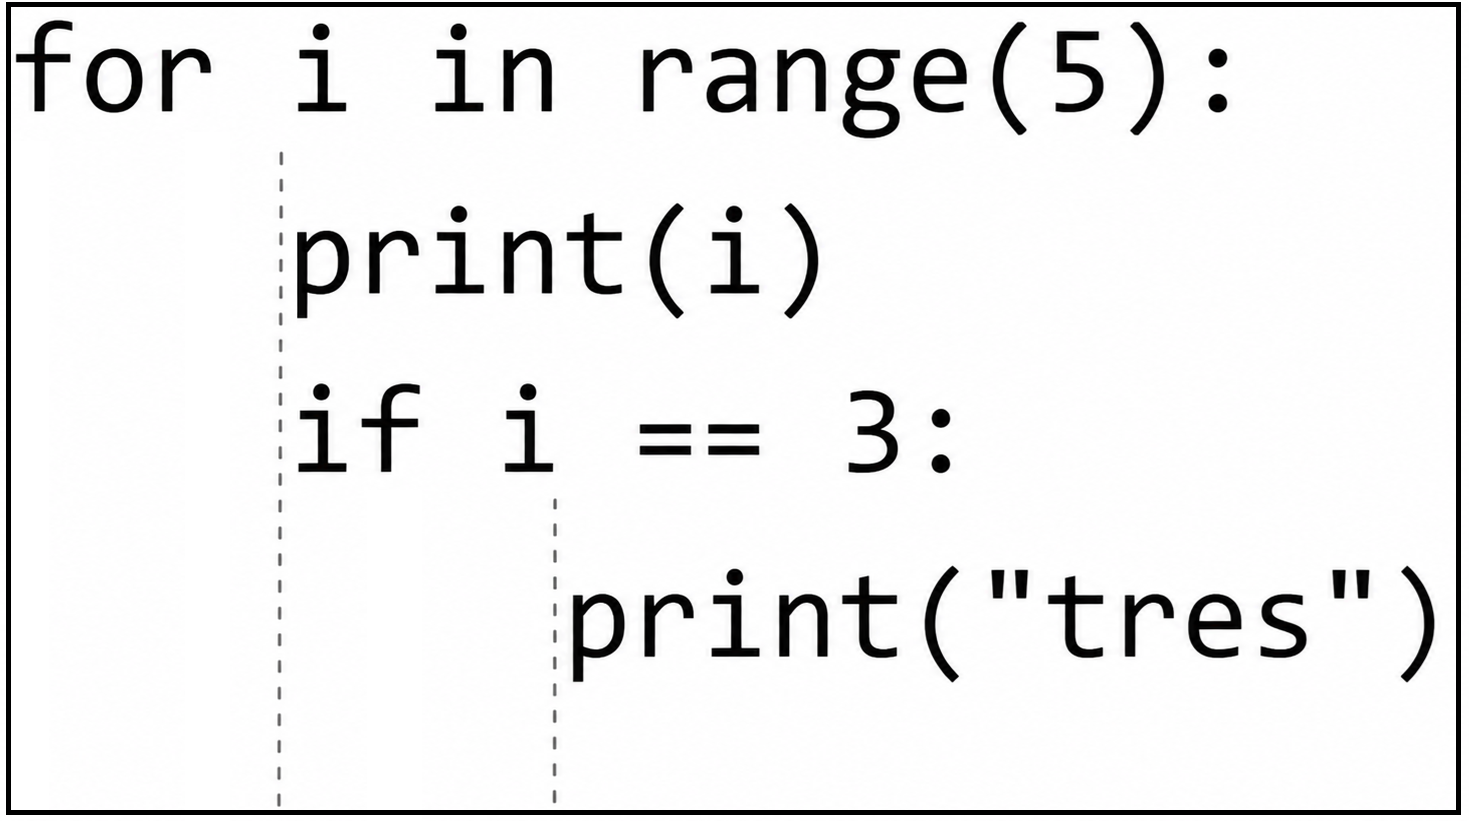
\includegraphics[width=\linewidth]{foto_ciclo_for_portada.png}
\end{minipage}
\end{formulabox}

% =========================================
% PRÁCTICA GUIADA
% =========================================
\newpage
\section*{Práctica Guiada --- se resuelve en conjunto}

\subsubsection*{Torneo de videojuegos --- el puntaje más alto}
Un torneo de videojuegos registra los puntajes de la ronda de clasificación. Cada jugador ingresa su puntaje, uno por uno, y el sistema debe seguir recibiendo puntajes hasta que se ingresa \textbf{-1}, que marca el fin de la ronda. Al terminar, el sistema debe informar cuál fue el \textbf{puntaje más alto} registrado en toda la ronda.

\textbf{El programa debe:}
\begin{itemize}
  \item Pedir puntajes repetidamente con \texttt{while}, hasta recibir \texttt{-1}.
  \item Ir comparando cada puntaje ingresado con el más alto registrado hasta el momento, y quedarse con el mayor.
  \item Imprimir el puntaje más alto al terminar.
  \item Si el primer ingreso ya es \texttt{-1} (no se registró ningún puntaje), informar que no hubo puntajes, sin mostrar un máximo.
\end{itemize}

\noindent{\footnotesize\textit{\textbf{Pista --- Cómo partir el máximo:} Antes de tener ningún puntaje, todavía no existe un ``máximo''. Puedes usar el primer puntaje válido que se ingrese como punto de partida, y desde ahí ir comparando los que vengan después.}}

\vspace{1mm}
{\footnotesize
\renewcommand{\arraystretch}{0.85}
\setlength{\tabcolsep}{4pt}
\noindent\begin{tabularx}{\linewidth}{|Y|Y|}
\hline
\textbf{Ejemplo 1} & \textbf{Ejemplo 2} \\
\hline
\textbf{Entrada:} \texttt{850}, \texttt{1200}, \texttt{690}, \texttt{-1} & \textbf{Entrada:} \texttt{-1} \\
\hline
\textbf{Salida:} \texttt{Puntaje más alto: 1200} & \textbf{Salida:} \texttt{No se registró ningún puntaje.} \\
\hline
\end{tabularx}
}

\vspace{2mm}\textit{Escribe el programa acordado en clase aquí:}
\begin{cajaescribe}[height=8.5cm]
\end{cajaescribe}

% =========================================
% SECCIÓN 1
% =========================================
\newpage
\section*{Sección 1 --- Ítems cortos}
Repaso rápido de ciclos, dividido en dos partes.

\subsection*{1A --- Arma el código}
Completa la parte marcada con líneas en blanco (\_\_\_\_) para que el programa haga lo que pide la narrativa. Escribe directamente sobre la línea, en el mismo bloque de código.

\subsubsection*{Ítem 1A.1}
La radio escolar transmite un anuncio publicitario cada 3 minutos, desde el minuto 0 hasta el minuto 21 de un bloque de transmisión. El programa debe imprimir en qué minutos se transmite un anuncio.

\begin{cajacodigo}
\begin{Verbatim}[fontsize=\small]
for minuto in ________________________________:
    print("Anuncio en el minuto", minuto)
\end{Verbatim}
\end{cajacodigo}

\noindent{\footnotesize\textit{\textbf{Pista:} Un \texttt{range()} de tres números es \texttt{range(inicio, fin, paso)} --- recuerda que el fin queda excluido, así que debe ser un número más que el último minuto que quieres incluir.}}

\subsubsection*{Ítem 1A.2}
El sistema de un parque de diversiones revisa las atracciones numeradas del 1 al 12, buscando la primera que tiene mantenimiento programado: la atracción N°9. Apenas la encuentra, debe avisar cuál es y \textbf{detener la búsqueda de inmediato}, sin seguir revisando las que quedan.

\begin{cajacodigo}
\begin{Verbatim}[fontsize=\small]
for atraccion in range(1, 13):
    if atraccion == 9:
        print("Atracción en mantenimiento: N°", atraccion)
        ________________________________________________
\end{Verbatim}
\end{cajacodigo}

\noindent{\footnotesize\textit{\textbf{Pista:} Piensa en la instrucción que corta un ciclo de inmediato, sin esperar a que termine de recorrer los valores que quedan.}}

\newpage
\subsection*{1B --- Arregla el bug}
Cada fragmento tiene un solo error. Reescribe el código \textbf{corregido y completo} en el espacio en blanco debajo de cada uno.

\subsubsection*{Ítem 1B.1}
Un campamento de verano organiza 3 cabañas con 4 actividades cada una. El sistema debe imprimir cada actividad de cada cabaña, pero algo salió mal: solo se imprime la última actividad de cada cabaña.

\begin{cajacodigo}
\begin{Verbatim}[fontsize=\small]
for cabana in range(1, 4):
    for actividad in range(1, 5):
        numero_actividad = actividad
    print("Cabaña", cabana, "- Actividad", numero_actividad)
\end{Verbatim}
\end{cajacodigo}
\noindent{\footnotesize\textit{\textbf{Pista:} Cuenta cuántas veces se ejecuta el \texttt{print()} tal como está escrito, y compáralo con cuántas veces debería ejecutarse según el enunciado.}}

\vspace{1mm}\textit{Código corregido:}
\begin{cajaescribe}[height=3.5cm]
\end{cajaescribe}

\subsubsection*{Ítem 1B.2}
Una app de estudio revisa 8 flashcards numeradas del 1 al 8 y debe contar cuántas son de \textbf{repaso rápido}: las de número \textbf{par}. Las impares se saltan con \texttt{continue}. Pero el contador de repaso rápido nunca sube como corresponde --- siempre termina en 8.

\begin{cajacodigo}
\begin{Verbatim}[fontsize=\small]
contador_repaso_rapido = 0

for numero_flashcard in range(1, 9):
    contador_repaso_rapido = contador_repaso_rapido + 1
    if numero_flashcard % 2 != 0:
        continue

print("Repaso rápido:", contador_repaso_rapido)
\end{Verbatim}
\end{cajacodigo}
\noindent{\footnotesize\textit{\textbf{Pista:} Revisa el orden: ¿la línea que suma el contador se ejecuta antes o después de que el programa decida si esa flashcard se salta?}}

\vspace{1mm}\textit{Código corregido:}
\begin{cajaescribe}[height=3.5cm]
\end{cajaescribe}

% =========================================
% SECCIÓN 2 --- una plana por ejercicio
% =========================================
\newpage
\section*{Sección 2 --- Programas completos}
Programas completos desde una narrativa. El Ejercicio 2 pide sus datos con \texttt{input()} --- lee bien el tipo de dato que se espera antes de escribir tu código.

\subsubsection*{Ejercicio 1 --- Feria de talentos}
La feria de talentos del liceo tiene 4 bloques de presentaciones. El bloque $i$ tiene $i$ presentaciones, y cada presentación dura 8 minutos. El programa debe calcular el \textbf{total de minutos} de presentaciones en toda la feria, y además contar en \textbf{cuántos bloques se superaron los 24 minutos} de duración.

\textbf{El programa debe:}
\begin{itemize}
  \item Usar \texttt{bloques\_totales = 4}.
  \item Para cada bloque (empezando en 1), calcular los minutos de ese bloque sumando 8 minutos por cada presentación que le corresponde, y acumular ese subtotal en el total general de la feria.
  \item Contar en cuántos bloques la duración del bloque superó los 24 minutos (estrictamente mayor).
  \item Imprimir el total de minutos de toda la feria y la cantidad de bloques que superaron los 24 minutos, cada uno con su etiqueta.
\end{itemize}

\noindent{\footnotesize\textit{\textbf{Pista 1 --- Reinicia el contador de minutos en cada bloque:} Antes de empezar a contar las presentaciones de un bloque nuevo, la variable que acumula los minutos de ese bloque debe volver a partir en 0.}}

\noindent{\footnotesize\textit{\textbf{Pista 2 --- El contador de bloques se revisa después del ciclo interno:} Recién cuando terminaste de sumar todas las presentaciones de un bloque sabes si ese bloque superó los 24 minutos.}}

\vspace{1mm}\textbf{El programa imprime:}
\begin{cajacodigo}
\begin{Verbatim}[fontsize=\small]
Total de minutos de la feria: 80
Bloques que superaron los 24 minutos: 1
\end{Verbatim}
\end{cajacodigo}

\vspace{1mm}\textit{Escribe tu programa aquí:}
\begin{cajaescribe}[height=8.5cm]
\end{cajaescribe}

\newpage
\subsubsection*{Ejercicio 2 --- Invernadero escolar}
Un invernadero escolar registra la temperatura de sus primeros 6 sensores del día, ingresada manualmente uno por uno. El programa debe contar cuántas lecturas fueron \textbf{``normales''} (entre 18 y 28 grados, ambos límites incluidos) y cuántas fueron \textbf{``de alerta''} (fuera de ese rango).

\textbf{El programa debe:}
\begin{itemize}
  \item Usar un \texttt{for} con \texttt{range(6)} para repetir exactamente 6 veces.
  \item Por cada vuelta, pedir la temperatura del sensor correspondiente con \texttt{input()} (puede tener decimales).
  \item Clasificar cada lectura como normal o de alerta, según el rango indicado.
  \item Imprimir ambos conteos al terminar, cada uno con su etiqueta.
\end{itemize}

\noindent{\footnotesize\textit{\textbf{Pista 1 --- Dos contadores, uno por categoría:} Necesitas una variable que cuente las lecturas normales y otra distinta que cuente las de alerta --- cada lectura suma a una sola de las dos.}}

\noindent{\footnotesize\textit{\textbf{Pista 2 --- Ambos límites incluidos:} Una lectura de exactamente 18 o exactamente 28 grados cuenta como normal, no como de alerta.}}

\vspace{1mm}
{\footnotesize
\renewcommand{\arraystretch}{0.85}
\setlength{\tabcolsep}{4pt}
\noindent\begin{tabularx}{\linewidth}{|Y|Y|}
\hline
\textbf{Ejemplo 1} & \textbf{Ejemplo 2} \\
\hline
\textbf{Entrada:} \texttt{20}, \texttt{30}, \texttt{18}, \texttt{28}, \texttt{15}, \texttt{22} & \textbf{Entrada:} \texttt{15}, \texttt{35}, \texttt{20}, \texttt{25}, \texttt{10}, \texttt{40} \\
\hline
\textbf{Salida:} \texttt{Lecturas normales: 4} \newline \texttt{Lecturas de alerta: 2} & \textbf{Salida:} \texttt{Lecturas normales: 2} \newline \texttt{Lecturas de alerta: 4} \\
\hline
\end{tabularx}
}

\vspace{1mm}\textit{Escribe tu programa aquí:}
\begin{cajaescribe}[height=8.5cm]
\end{cajaescribe}

\end{document}
